\documentclass[norsk,a4paper,12pt]{article} 
\usepackage[norsk]{babel} 
\usepackage[T1]{fontenc} %for å bruke æøå 
\usepackage[utf8x]{inputenc} 
\usepackage{graphicx} %for å inkludere grafikk 
\usepackage{verbatim} %for å inkludere filer med tegn LaTeX ikke liker 
\usepackage{amsfonts} 
\usepackage{amsmath} 
\usepackage{amssymb} 
%\usepackage{savesym} 
%\savesymbol{square} 
\bibliographystyle{plain} 
\usepackage{float} 
%\usepackage{SIunits} 
\usepackage{textcomp} 
\usepackage{parskip} 
\usepackage{array} 
%\usepackage[framed]{mcode} 
\usepackage[margin=2.3cm]{caption}
\usepackage{listings}

\begin{document}

\title{AST5220 Cosmology II: Milestone 4}
\author{Peder Forfang}
\maketitle


\section{The CMB power spectrum}

Earlier we have studied several physical quantities in our universe, such as matter and energy components, optical depth, density perturbations and gravitational potentials. We have seen how they evolve as the universe expands from a time just beyond inflation until today. We have what we need to construct the power spectrum of the CMB and that is what this final part is all about. When we study the CMB we look at the temperature field we see around us today. The spherical harmonics transform of the CMB temperature field is

\begin{equation}
 T(n) = \sum_{lm} a_{lm}Y_{lm}(n)
\end{equation}

where $Y_{lm}$ are the spherical harmonics and $a_{lm} $ are the spherical harmonics coefficients. The CMB power spectrum is defined as the expectation value of the square of these coefficients. 

\begin{equation}
 Cl\equiv \langle|a_{lm}|^2\rangle = \langle a_{lm}a_{lm}^*\rangle
\end{equation}

We assume the universe is isotropic. In other words the power spectrum is the same in all directions. Thus we have no $m$ dependence in the power spectrum. Earlier in the project we computed the temperature field in the form $ \Theta_l(k,x)$, however only up to $l=6$ and we need about $l = 1200$. To save time we will use the ``line of sight integration approach''. The basic idea is that instead of first expanding in multipoles then integrating the equations, we do it in reverse. The final expression of the temperature field today is simply

\begin{equation}
 \Theta_l(k,x=0) = \int_{-\infty}^0 S(k,x)j_l[k(\eta_0-\eta)]dx
\end{equation}

where $j_l$ are the spherical Bessel functions and the source function $S(k,x)$ is defined as

\begin{equation}
 S(k,x) = g\bigg[\Theta_0 + \Psi + \frac{1}{4}\Pi \bigg] + e^{-\tau}[\Psi' - \Phi']-\frac{1}{k}\frac{d}{dx}(H_pgv_b) + \frac{3}{4k^2}\frac{d}{dx}\bigg[H_p\frac{d}{dx}(H_pg\Phi)\bigg]
\end{equation}

where, in this case, $\Pi = \Theta_2$. The other quantities are computed earlier in this project. In the first term, $\Theta_0$ is the CMB monopole radiation we observe today, weighted by the visibility function, g. The other sub-terms are corrections to this effect. The photons have to climb out of a gravitational potential, and loses energy. This is accounted for by $Psi$. $\Pi$ is a small quadrupolar correction to the original monopole contribution. Next we have the integrated Sachs-Wolf term, which describes how gravitational potentials change while the photons are moving.

So far so good, we are now ready to compute $C_l$ with $\Theta_l(k)$ as our coefficients. Earlier in this project we originally set $ \Phi = 1$ to simplify calculations. To correct this we will multiply with the primordial power spectrum $ P(k)$ coming from inflation. 

\begin{equation}
 C_l = \int \frac{d^3k}{(2\pi)^3}P(k)\Theta_l^2(k)
\end{equation}

$P(k)$ can be predicted by a Harrison-Zel'dovich spectrum

\begin{equation}
 \frac{k^3}{2\pi^2}P(k) = \bigg ( \frac{ck}{H_0} \bigg )^{n-1}
\end{equation}

where $n = 0.96$ is the spectral index. Our final expression becomes

\begin{equation}
 C_l = \int_0^{\infty} \bigg ( \frac{ck}{H_0} \bigg )^{n-1} \Theta_l^2(k) \frac{dk}{k}
\end{equation}

We would try to get results similar to the observed values. As a test we can compare and try to fit it to data obtained from Planck Legacy Archive. 




\begin{figure}[H] 
\begin{center} 
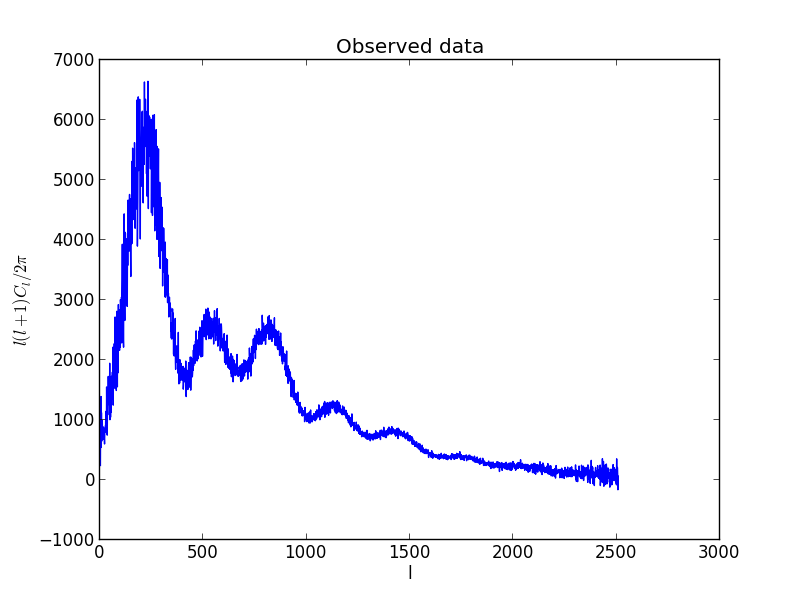
\includegraphics[scale=0.5]{plank_data.png} 
 

\caption{Power spectrum obtained from Planck Legacy Archive.} 
\end{center} 
\end{figure}

However, due to some unresolved technical issues, I could not produce results even close to the Planck spectrum. I found that while calculating the spherical Bessel functions something beyond my comprehension went terribly wrong. Because of this I did not get the results I was hoping for. The source code is attached to the report in case future readers might solve the mystery. The figures below shows what results I did produce (although they are not quite right). 

\begin{figure}[H] 
\begin{center} 
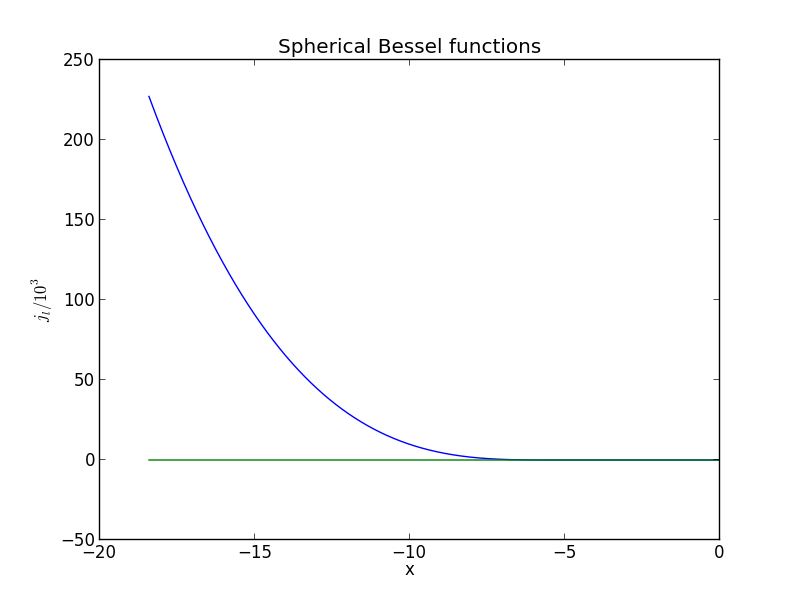
\includegraphics[scale=0.5]{j_l.png} 
 

\caption{Bessel function for different $l$ and $k = 4.84e-24$ . I believe this is the source of my numerical problems.} 
\end{center} 
\end{figure}


\begin{figure}[H] 
\begin{center} 
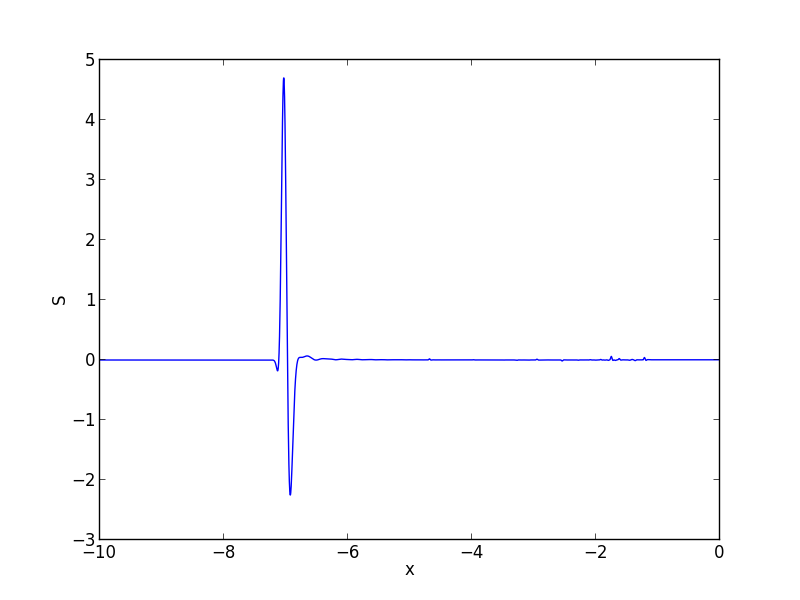
\includegraphics[scale=0.5]{s.png} 
 

\caption{The source function $S(x,k)$ for the same $k$ .} 
\end{center} 
\end{figure}


\begin{figure}[H] 
\begin{center} 
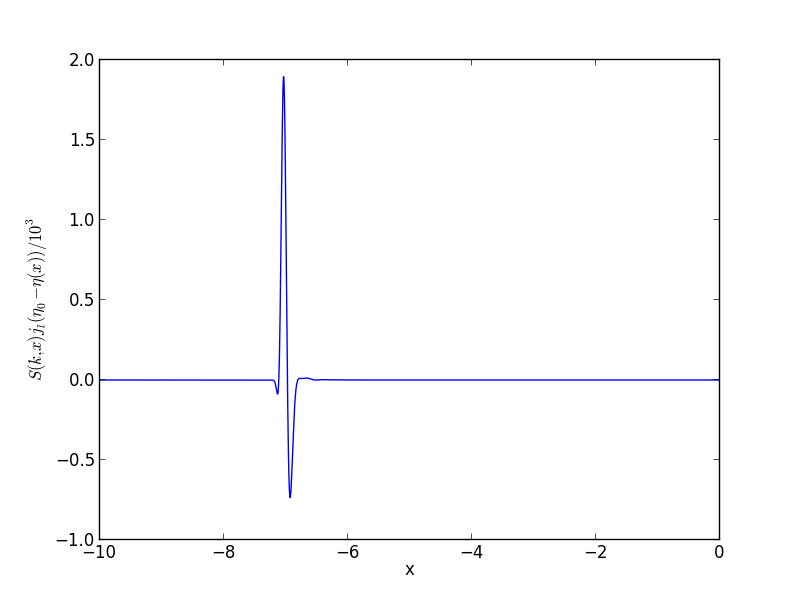
\includegraphics[scale=0.5]{sj.png} 
 

\caption{The figure shows the source fuction times $j_l$. It looks almost the same as the source function in the plot above. Oscillations towards $x = 0$ caused by Bessel functions would be expected.} 
\end{center} 
\end{figure}

\begin{figure}[H] 
\begin{center} 
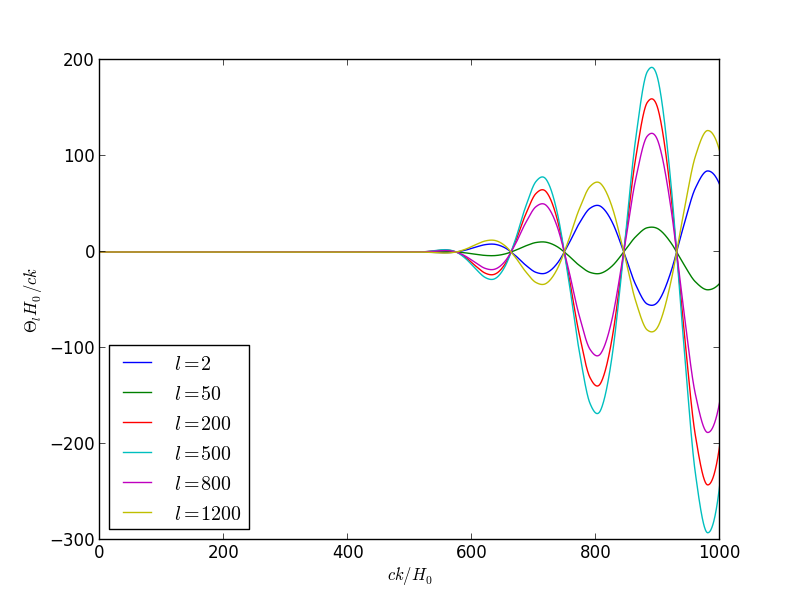
\includegraphics[scale=0.5]{theta.png} 
 

\caption{The transfer function $\Theta_l(k)$ for six different $l$.} 
\end{center} 
\end{figure}


\begin{figure}[H] 
\begin{center} 
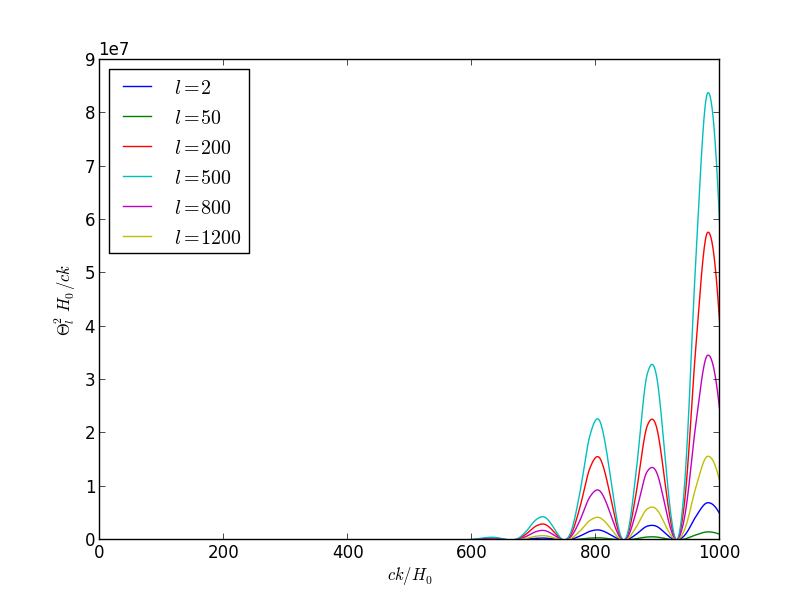
\includegraphics[scale=0.5]{theta2.png} 
 

\caption{The spectrum integrand $\Theta_l(k)^2 / k$ for six different $l$.} 
\end{center} 
\end{figure}

And for the Grand Finale, the CMB power spectrum:


\begin{figure}[H] 
\begin{center} 
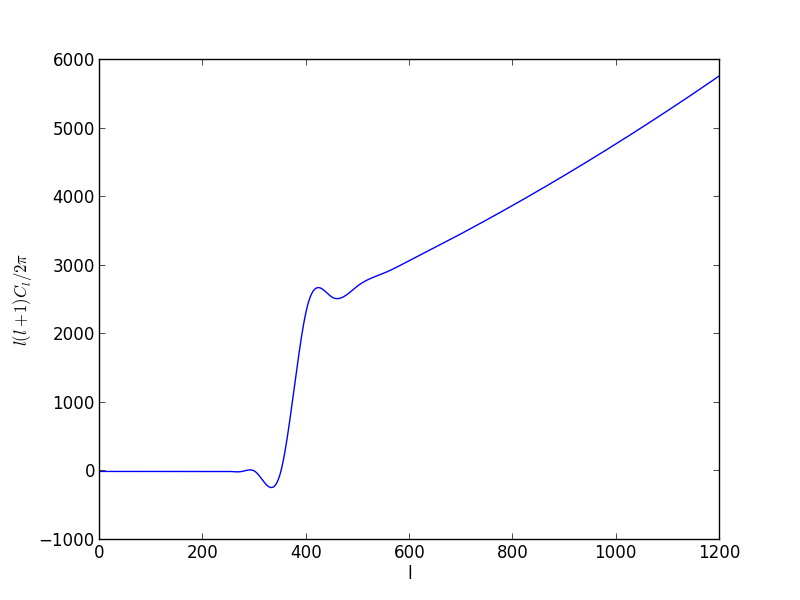
\includegraphics[scale=0.5]{cl.png} 
 

\caption{The numerically computed CMB power spectrum $C_l$.} 
\end{center} 
\end{figure}



\end{document}